\subsection{Distribution Layer}
\emph{author: Emanuel Kranjec}\bigskip

To ensure simple and efficient data lookups CockroachDB provides a monolithic sorted map of key-value pairs. Those key-value
pairs include two fundamental elements. One stores the meta range and the other the table data.

\begin{figure}[H]
    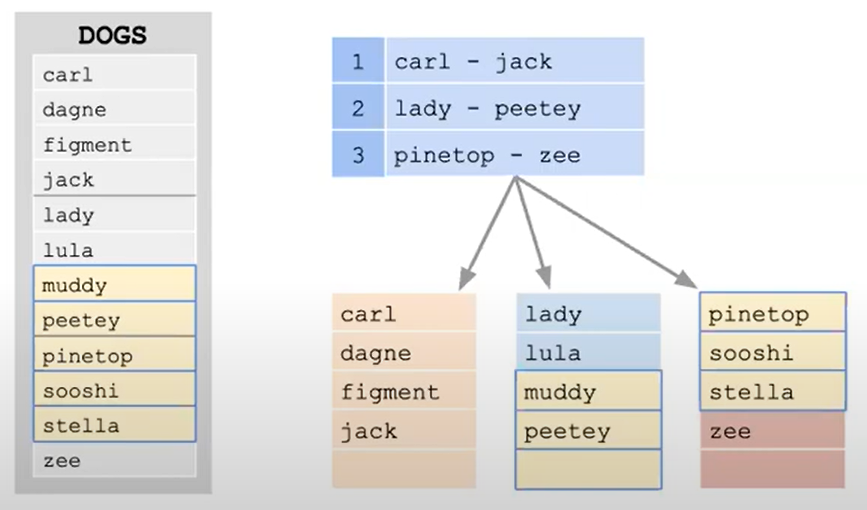
\includegraphics[width=\textwidth]{kv-store}
    \caption{Simplified example of key-values for particular ranges}
    \label{fig:kv-store}
\end{figure}

\paragraph{Meta ranges}
describe the location of data including all of its replicas in the cluster.

\paragraph{Table data}
describes the rows of a table included in this particular range.
